% !TEX root = ../supp.tex

\section*{C. Additional Analysis}
\label{sec:C}
We conduct additional experiments for further analysis of the proposed method. In the following experiments, we evaluate our models on the Breakfast dataset with two observed ratios $\alpha \in \{0.2, 0.3\}$. Unless otherwise specified, all experimental settings are the same as those in Sec. 5.4.

\begin{table}[t]
\begin{center}
\renewcommand{\arraystretch}{0.8}
\scalebox{0.62}{
\begin{tabular}{wl{1.8cm}C{1cm}C{0.8cm}C{0.8cm}C{0.8cm}C{0.8cm}C{0.8cm}C{0.8cm}C{0.8cm}C{0.8cm}}
\toprule
\multirow{2}*[-0.5ex]{method} &\multirow{2}*[-0.5ex]{input} &\multicolumn{8}{c}{$\beta~(\alpha=0.2$)}\\
\cmidrule{3-10}
& &0.01 & 0.02 & 0.03 & 0.05& 0.1 & 0.2 & 0.3 & 0.5 \\
\cmidrule{1-10}
AVT~\cite{girdhar2021anticipative}&ViT&30.25 & 30.24 & 25.72 & 21.87& 14.22 & 10.69 & 8.49 & 5.83 \\
% ViT&AVT~[17]& 14.22 & 10.69 & 8.49 & 5.83 & \\
% I3D&AVT~[17]& 17.84 & 13.20 & 9.01 & 4.61 & 14.92 & 12.79 & 10.38 & 5.81\\
AVT~\cite{girdhar2021anticipative}&I3D& 26.13 & 22.03 & 20.24 & 13.52 & 17.84 & 13.20 & 9.01 & 4.61\\
% \ccol I3D&\ccol\textbf{\ours~(10f)}  &\ccol \textbf{68.18} & \ccol \textbf{51.68} &\ccol \textbf{45.82} &\ccol \textbf{40.94}   &\ccol \textbf{37.43} & \ccol \textbf{26.27} & \ccol \textbf{21.46} & \ccol \textbf{13.22} \\
\ccol\textbf{\ours~(ours)} &\ccol I3D &\ccol \textbf{51.16} & \ccol \textbf{44.34} &\ccol \textbf{40.84} &\ccol \textbf{40.56}   &\ccol \textbf{39.43} & \ccol \textbf{27.54} & \ccol \textbf{23.31} & \ccol \textbf{17.77} \\
\midrule
&&\multicolumn{8}{c}{$\beta~(\alpha=0.3$)}\\
\midrule
% $\beta$ &model& 
% \cmidrule[0.5pt]( r){1-6}
% \cmidrule[0.5pt]( l){7-10}
AVT~\cite{girdhar2021anticipative}&ViT & 30.93 & 30.62 & 27.85 & 23.60 & 18.28 & 13.51 & 9.65 & 7.35\\
AVT~\cite{girdhar2021anticipative}&I3D& 31.56 & 35.17 & 33.12 & 24.17 & 14.92 & 12.79 & 10.38 & 5.81\\
% \ccol I3D&\ccol\textbf{\ours~(10f)}     &\ccol \textbf{55.36} & \ccol \textbf{52.01} & \ccol \textbf{47.53} & \ccol \textbf{35.79} &\ccol \textbf{30.71} & \ccol \textbf{20.50} &\ccol \textbf{18.72} &\ccol \textbf{12.20}\\
\ccol\textbf{\ours~(ours)} &\ccol I3D  &\ccol \textbf{42.20} & \ccol \textbf{38.67} & \ccol \textbf{38.56} & \ccol \textbf{36.44} &\ccol \textbf{35.15} & \ccol \textbf{24.86} &\ccol \textbf{24.22} &\ccol \textbf{15.26}\\
\bottomrule
\end{tabular}
}
\end{center}
\vspace{-4mm}
\counterwithin{table}{section}
\renewcommand\thetable{S\arabic{table}}
\caption{\textbf{Performance comparison with AVT on 50Salads.} FUTR outperforms AVT especially when predicting long-term action sequences.}
\vspace{-4mm}
\label{tab:avt}
\end{table}

% wl{2.0cm}C{1.1cm}C{0.8cm}C{0.8cm}C{0.8cm}C{0.8cm}C{0.8cm}C{0.8cm}C{0.8cm}C{0.8cm}
\begin{figure}[t]
\vspace{3mm}
\centering
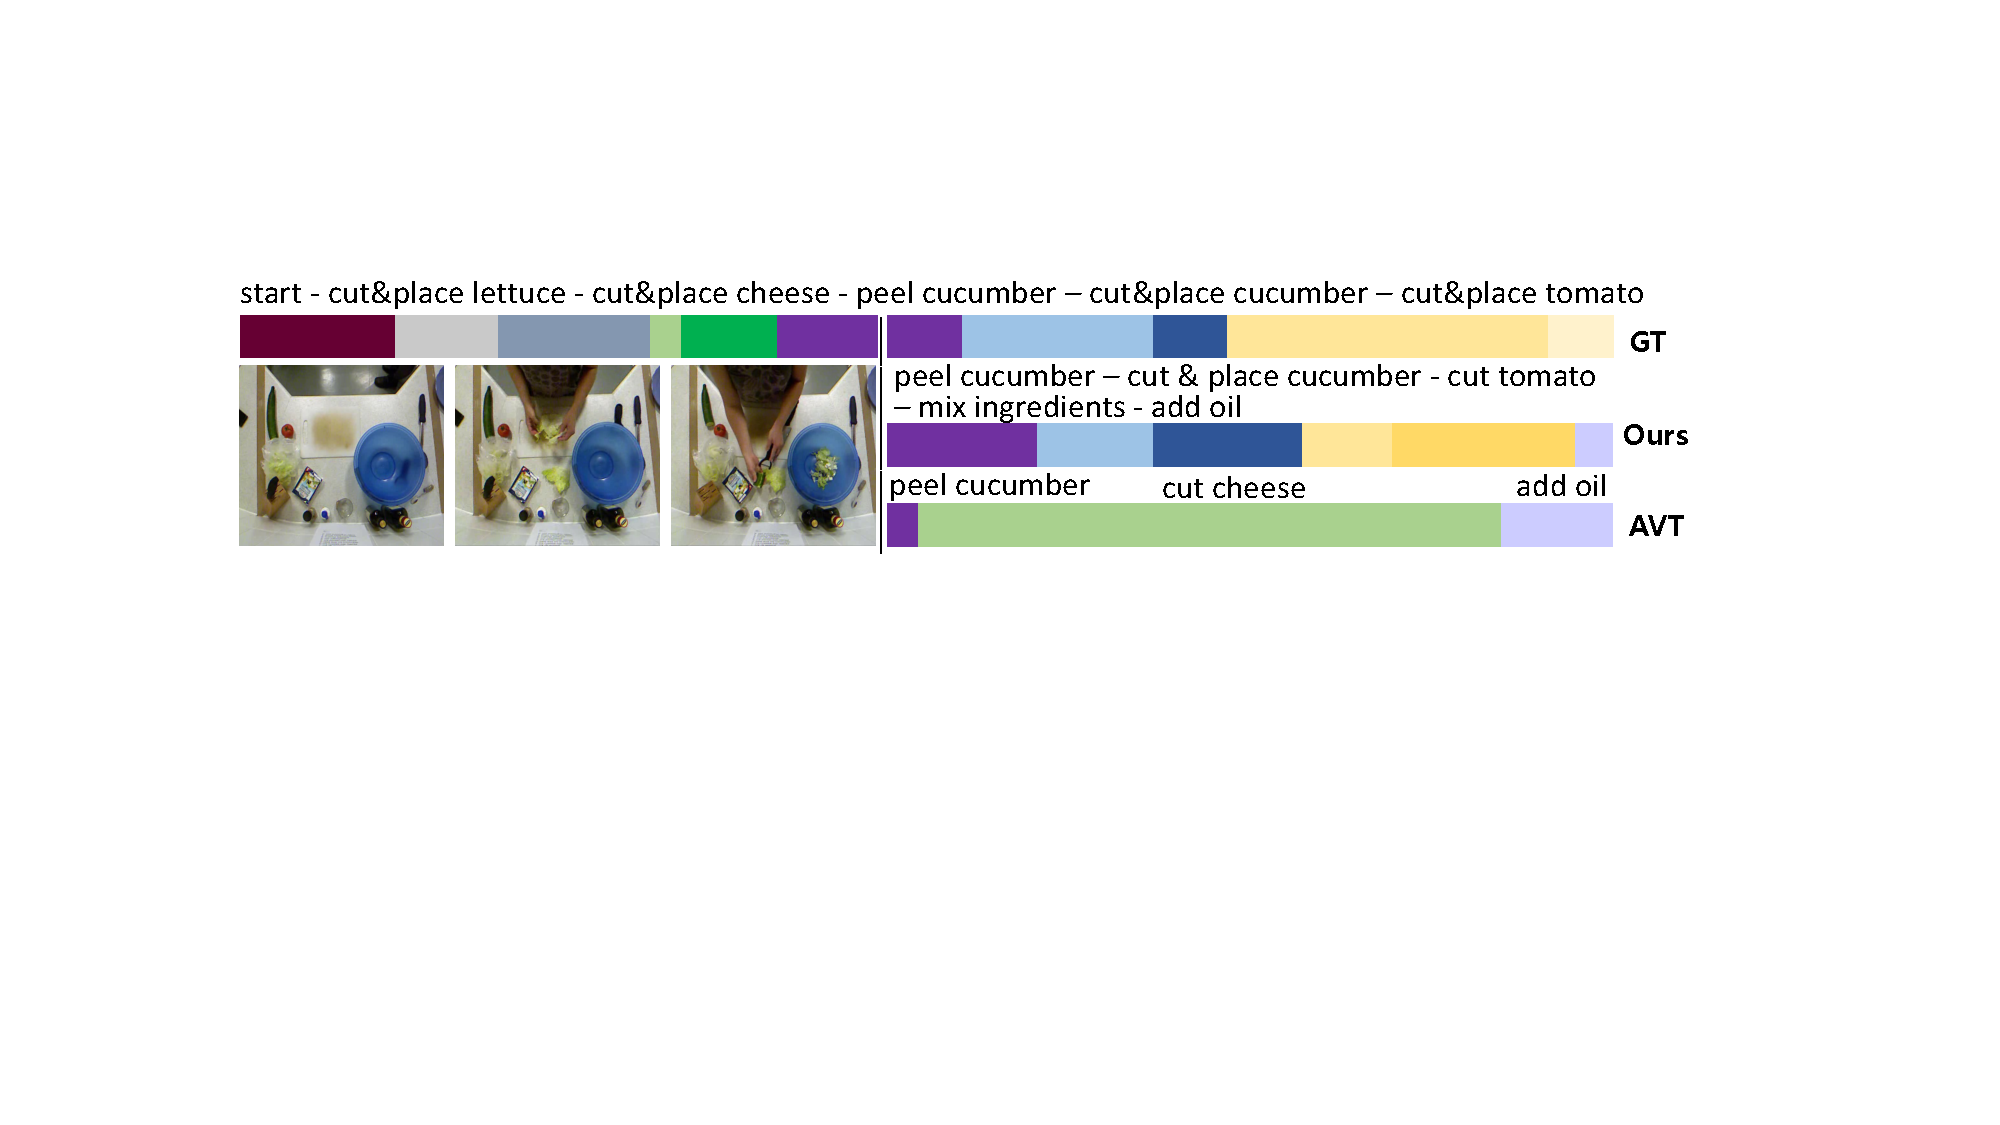
\includegraphics[width=\linewidth]{Figures/pdf/avt_qual2.pdf}
\counterwithin{figure}{section}
\renewcommand\thefigure{S\arabic{figure}}
\vspace{-6mm}
\caption{\textbf{Qualitative results of FUTR vs. AVT on 50Salads.} Each color in the color bar indicates an action label written above. AVT becomes inaccurate in the prolong predictions while our method is consistently accurate.}
\label{fig:avt}
% \vspace{-3mm}
\end{figure}
\begin{figure}[t]
    \vspace{-1mm}
    \centering
        \begin{minipage}{\linewidth}
            \begin{subfigure}{\linewidth}
                \centering
                \scalebox{0.82}{
                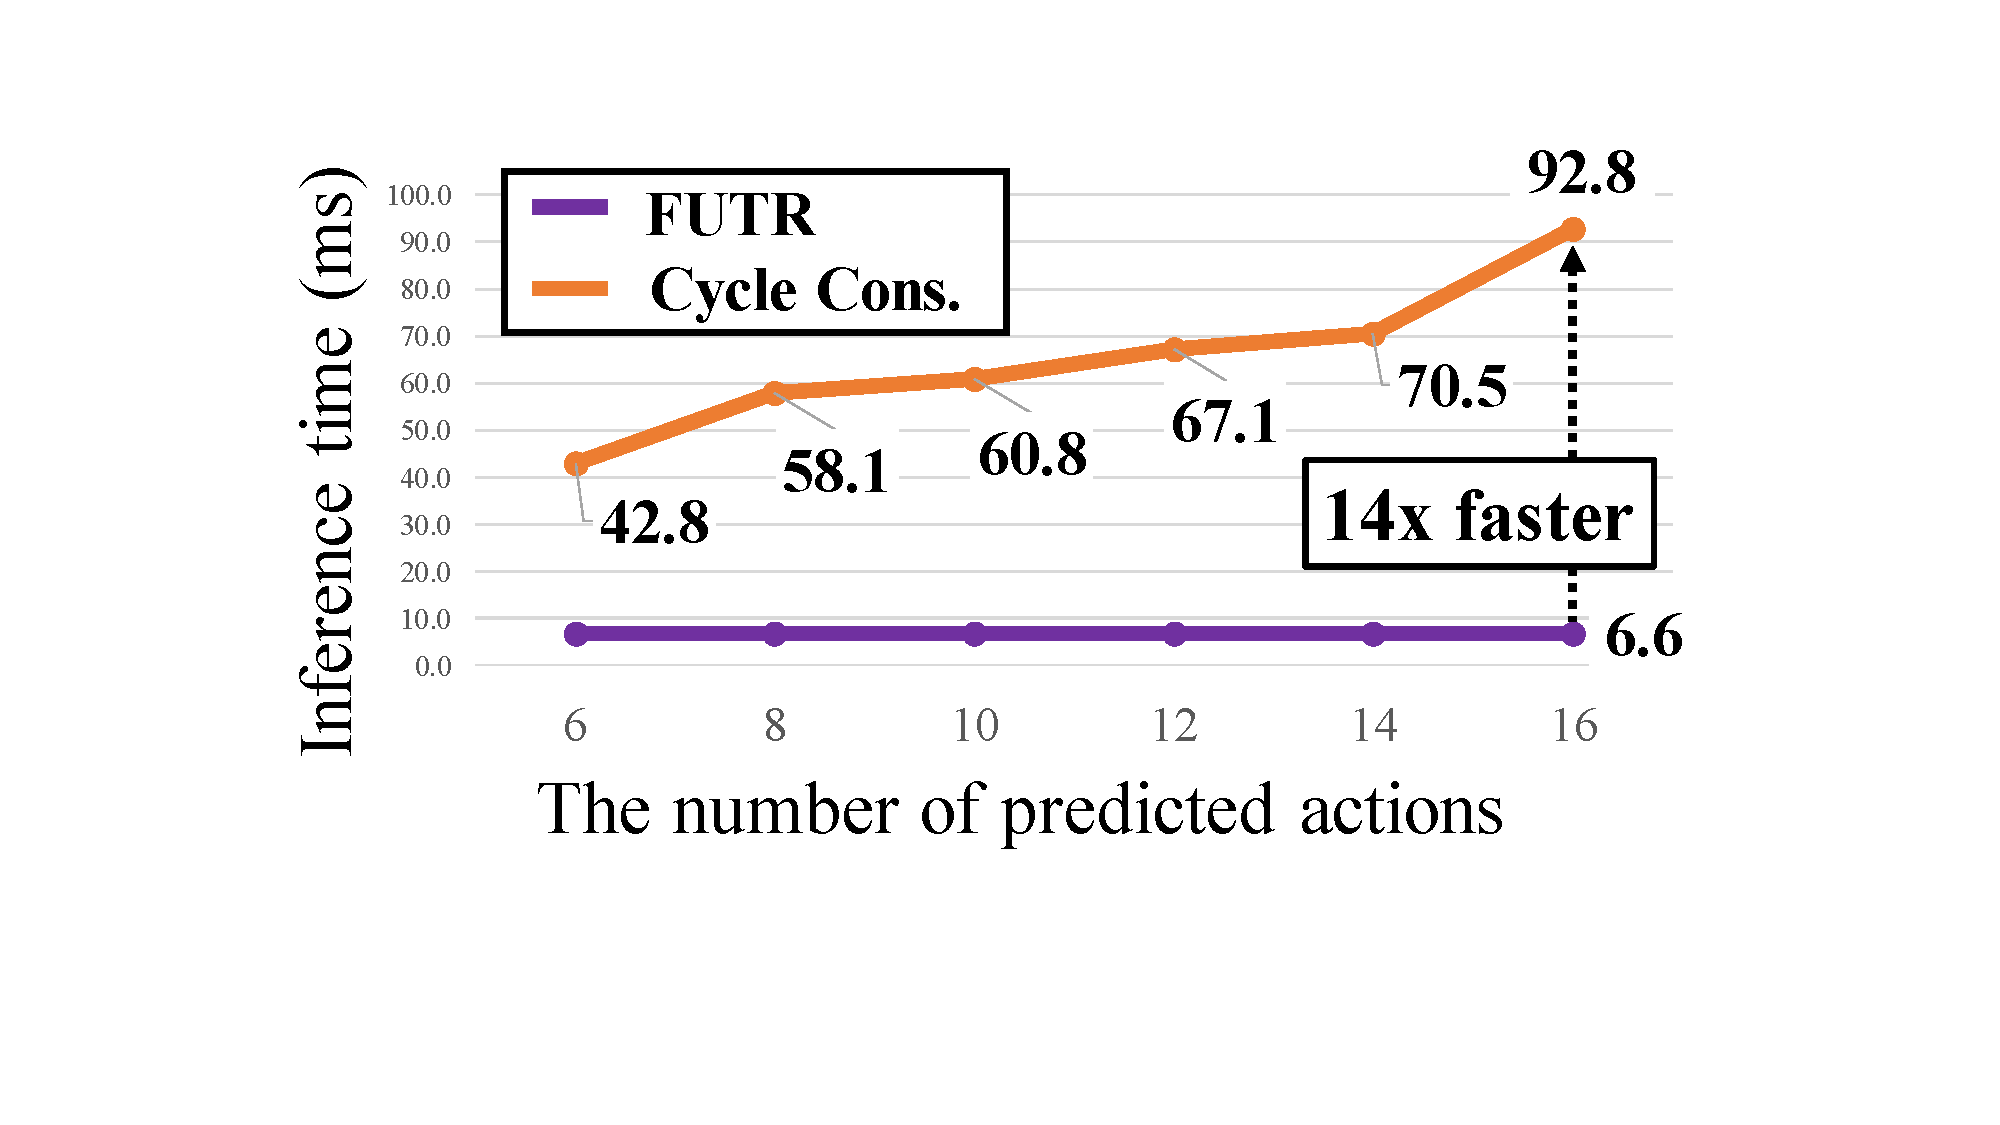
\includegraphics[width=\linewidth]{Figures/pdf/inf_cyc.pdf}
                }
                % \vspace{-5.5mm}
                \subcaption{\ours vs. Cycle Cons.~\cite{farha2020long}}
                \label{fig4:sub1}
            \end{subfigure}        
        \end{minipage}
        
        \vspace{2mm}
        
    \begin{minipage}{\linewidth}
            \begin{subfigure}{\linewidth}
                \centering
                \scalebox{0.8}{
                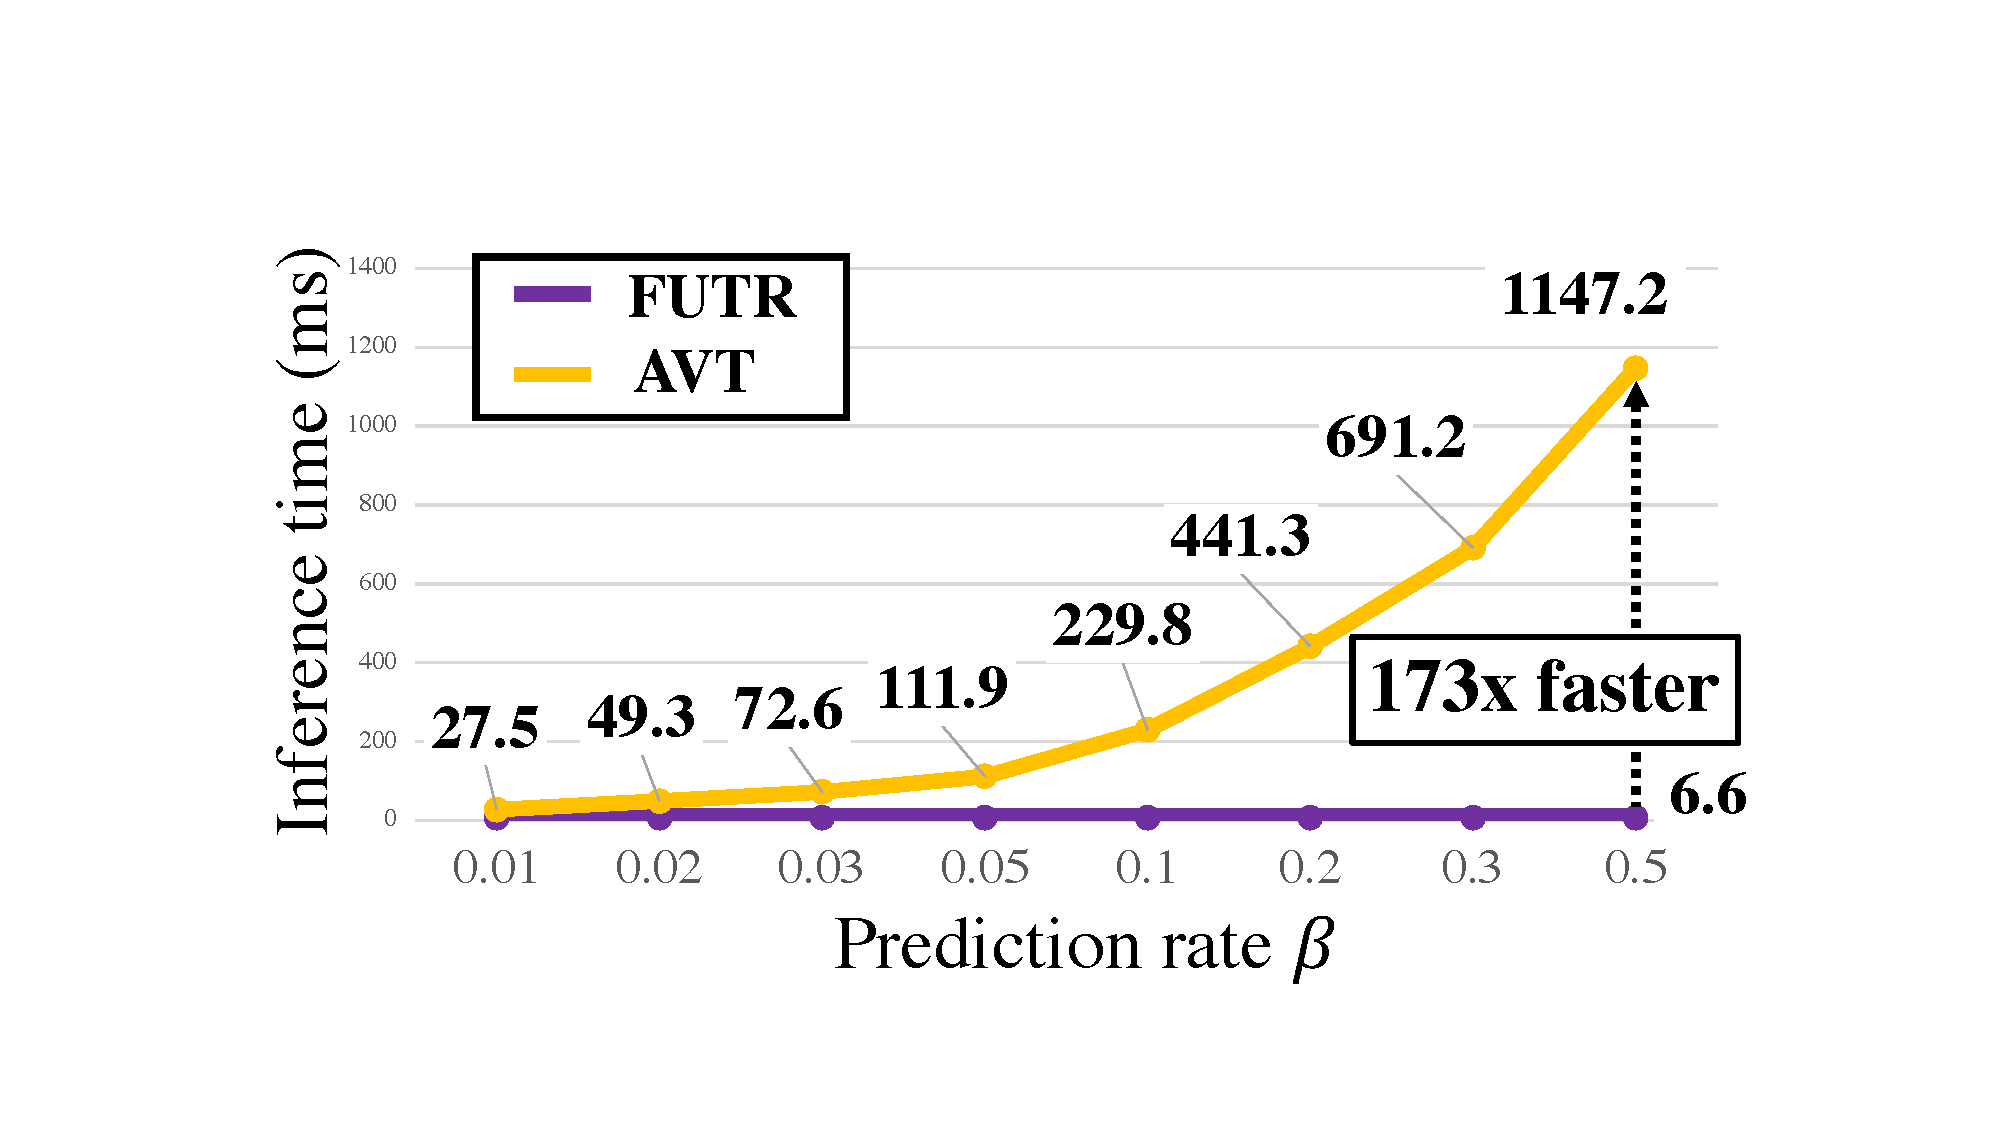
\includegraphics[width=\linewidth]{Figures/pdf/inf_avt.pdf}
                }
                % \vspace{-5.5mm}                
                \subcaption{\ours vs. AVT~\cite{girdhar2021anticipative}}
            \label{fig4:sub2}
            \end{subfigure}        
        \end{minipage}
    \vspace{-3.5mm}
    \counterwithin{figure}{section}
    \renewcommand\thefigure{S\arabic{figure}}
    \caption{\textbf{Inference time comparison with other methods}~\cite{farha2020long,girdhar2021anticipative}. Inference time of other methods linearly increases as the duration of the future action sequence to be predicted increases, \ie, the number of predicted actions or prediction rate $\beta$, increases, while that of FUTR is consistently fast.}
    \label{fig:inf}
    \vspace{-6mm}
\end{figure}

\begin{table*}[t]
\vspace{0mm}
\begin{center}
\scalebox{0.9}{
\begin{tabular}{C{1.8cm}C{1.1cm}C{1.1cm}C{1.1cm}C{1.1cm}C{1.1cm}C{1.1cm}C{1.1cm}C{1.1cm}}
            \toprule
            \multirow{2}*[-0.5ex]{$\gamma$} & \multicolumn{4}{c}{$\beta~(\alpha=0.2)$}&\multicolumn{4}{c}{$\beta~(\alpha=0.3)$} \\
            % \cmidrule[0.80pt]{1}
            \cmidrule(r){2-5}
            \cmidrule(l){6-9}
            & 0.1 & 0.2 & 0.3 & 0.5& 0.1 & 0.2 & 0.3 & 0.5  \\
            \midrule
            % 0.125 &  & &  & \\
            0.25 & 24.36 & 21.66 &  20.62 & 20.10 & 30.31 &27.53 & 25.45 & 23.19 \\
            0.5 & 25.26 & 22.99 &  22.10 & 21.37 & 31.14 &28.25 & 25.91 & 23.85 \\
            \ccolg 1 & \ccol\textbf{27.70} & \ccol\textbf{24.55} & \ccol\textbf{22.83} & \ccol\textbf{22.04}&\ccolg \textbf{32.27} & \ccolg \textbf{29.88} &  \ccolg \textbf{27.49} & \ccolg \textbf{25.87}\\
            \bottomrule
            \end{tabular}}
\end{center}
\vspace{-4mm}
\counterwithin{table}{section}
\renewcommand\thetable{S\arabic{table}}
\caption{\textbf{Effectiveness of global cross-attention.} We set observed ratio from the recent past as $\gamma$ to show the effectiveness of exploiting global cross-attention at long-term action anticipation. }
\vspace{-1mm}
\label{tab:sup_globality_full}
\end{table*}

% C{2cm}C{1.3cm}C{1.3cm}C{1.3cm}C{1.3cm}C{1.3cm}C{1.3cm}C{1.3cm}C{1.3cm}
% C{1cm}C{1cm}C{1cm}C{1cm}C{1cm}C{1cm}C{1cm}C{1cm}C{1cm}

% \begin{table}[t!]
% \begin{center}
% \scalebox{0.75}{
% \begin{tabular}{C{0.7cm}C{0.8cm}C{0.8cm}C{0.8cm}C{0.8cm}C{0.8cm}C{0.8cm}C{0.8cm}C{0.8cm}}
%             \toprule
%             \multirow{2}*[-0.5ex]{$\gamma$} & \multicolumn{4}{c}{$\beta~(\alpha=0.2)$}&\multicolumn{4}{c}{$\beta~(\alpha=0.3)$} \\
%             % \cmidrule[0.80pt]{1}
%             \cmidrule(r){2-5}
%             \cmidrule(l){6-9}
%             & 0.1 & 0.2 & 0.3 & 0.5& 0.1 & 0.2 & 0.3 & 0.5  \\
%             \midrule
%             % 0.125 &  & &  & \\
%             0.25 & 24.36 & 21.66 &  20.62 & 20.10 & 30.31 &27.53 & 25.45 & 23.19 \\
%             0.5 & 25.26 & 22.99 &  22.10 & 21.37 & 31.14 &28.25 & 25.91 & 23.85 \\
%             \ccolg 1 & \ccol\textbf{27.70} & \ccol\textbf{24.55} & \ccol\textbf{22.83} & \ccol\textbf{22.04}&\ccolg \textbf{32.27} & \ccolg \textbf{29.88} &  \ccolg \textbf{27.49} & \ccolg \textbf{25.87}\\
%             \bottomrule
%             \end{tabular}}
% \end{center}
% \vspace{-4mm}
% \counterwithin{table}{section}
% \renewcommand\thetable{S\arabic{table}}
% \caption{\textbf{Effectiveness of global cross-attention.} We set observed ratio from the recent past as $\gamma$ to show the effectiveness of exploiting global cross-attention at long-term action anticipation. }
% \vspace{-4mm}
% \label{tab:sup_globality_full}
% \end{table}
\begin{table*}[t!]
\vspace{1mm}
\begin{center}
\scalebox{0.9}{
\begin{tabular}{C{0.73cm}C{0.75cm}C{0.73cm}C{0.75cm}C{0.8cm}C{0.8cm}C{0.8cm}C{0.8cm}C{0.8cm}C{0.8cm}C{0.8cm}C{0.8cm}}
        \toprule
        \multicolumn{2}{c}{encoder}&\multicolumn{2}{c}{decoder} & \multicolumn{4}{c}{$\beta~(\alpha=0.2)$} & \multicolumn{4}{c}{$\beta~(\alpha=0.3)$}\\
        \cmidrule(r){1-2}
        \cmidrule{3-4}
        \cmidrule(l){5-8}
        \cmidrule(l){9-12}
        type&Loc.&type&Loc.& 0.1 & 0.2 & 0.3 & 0.5 & 0.1 & 0.2 & 0.3 & 0.5 \\
        \midrule
        -&-&learn&input& 21.79 & 20.14 & 19.88 & 18.25 & 26.53 &24.85 &25.04  &21.31 \\
        sine &input&learn&input& 21.29 & 19.55 & 19.11 & 18.23 & 27.40  &24.91 &24.13  &21.81\\
        learn &input&learn&input &23.79 & 21.37 & 20.49 & 19.62 & 30.80& 27.69 & 25.53 & 23.39\\
        % \cmidrule[0.5pt]{1-8}
        % learn &input&learn&attn. & 29.87& 26.32& 25.01 &22.87\\
        \ccolg learn &\ccolg attn.&\ccolg learn&\ccolg attn.& \ccol\textbf{27.70} & \ccol\textbf{24.55} & \ccol\textbf{22.83} & \ccol\textbf{22.04} & \ccolg\textbf{32.27} &\ccolg\textbf{29.88} & \ccolg\textbf{27.49} & \ccolg \textbf{25.87}\\
        \bottomrule
        \end{tabular}
        }
\vspace{-1mm}
\counterwithin{table}{section}
\renewcommand\thetable{S\arabic{table}}
\caption{\textbf{Position embedding analysis.} Adding learnable positional embeddings before every attention layer performs the best.
}
\label{tab:pos_full}
\end{center}
\vspace{-4mm}
\end{table*}
\begin{table*}[t!]
\begin{center}
\scalebox{0.9}{
\begin{tabular}{C{1.1cm}C{1.1cm}C{1.1cm}C{0.8cm}C{0.8cm}C{0.8cm}C{0.8cm}C{0.8cm}C{0.8cm}C{0.8cm}C{0.8cm}}
            \toprule
            \multicolumn{3}{c}{model} & \multicolumn{4}{c}{$\beta~(\alpha=0.2)$}&\multicolumn{4}{c}{$\beta~(\alpha=0.3)$} \\ 
            \cmidrule(r){1-3}
            \cmidrule{4-7}
            \cmidrule(l){8-11}
            $L^\mathrm{E}$&$L^\mathrm{D}$&$D$ & 0.1 & 0.2 & 0.3 & 0.5&0.1 & 0.2 & 0.3 & 0.5 \\
            \midrule
            1&1& 128 &24.02&21.00& 19.71 & 19.39 & 29.38 &26.51 & 25.06 & 23.83 \\
            \ccolg 2&\ccolg 1& \ccolg 128 & \ccol\textbf{27.70} & \ccol\textbf{24.55} & \ccol22.83 &\ccol\textbf{22.04}& \ccolg 32.27 & \ccolg \textbf{29.88} &  \ccolg27.49 & \ccolg \textbf{25.87}\\
            % 2&2& 128 & 30.38 & 27.83 & 26.08 & 24.25\\
            3&1& 128 & 24.78 & 22.78 & 21.46 & 20.53 & 30.44 & 27.61 & 25.73 & 23.75\\
            3&2& 128 & 26.72 & 23.82 & 22.57 & 21.29 & 32.55 & 29.20 & 26.59 & 24.92\\
            3&3& 128 & 26.68 & 23.41 & 22.14 & 21.56 & \textbf{33.06} & 29.14 & \textbf{28.12} & 24.93\\
            4&4& 128 & 26.77 & 23.60 & 22.92 & 21.24 & 31.35 & 28.58 & 27.04 & 24.73\\
            5&5& 128 & 26.75 & 24.23 & \textbf{23.55} & 21.16 & 32.68 & 29.38 & 28.05 & 24.89\\
            \midrule
            2&1& 64 & 24.78 & 21.81 & 20.56 & 19.88 & 29.92 & 27.03& 26.29 & 23.53\\
            2&1& 256 & 24.56 & 21.62 & 21.35 & 19.41 & 31.19 & 26.03 & 26.07 & 24.29\\
            2&1& 512 & 19.82 & 17.50 & 18.07 & 16.31 & 23.68 & 22.18 & 23.57 & 22.56\\
            \bottomrule
            \end{tabular}}
\end{center}
\vspace{-5mm}
\counterwithin{table}{section}
\renewcommand\thetable{S\arabic{table}}
\caption{\textbf{Model analysis.} We study the number of encoder layers $L^\textrm{E}$, the number of decoder layers $L^\textrm{D}$, and hidden dimension $D$ of our model. We show the robustness of our methods over the number of layers, and find that the optimal hidden dimension $D$ is 128. }
\vspace{0mm}
\label{tab:model_full}
\end{table*}

% \begin{table}[t!]
% \begin{center}
% \scalebox{0.65}{
% \begin{tabular}{C{0.5cm}C{0.5cm}C{0.7cm}C{0.8cm}C{0.8cm}C{0.8cm}C{0.8cm}C{0.8cm}C{0.8cm}C{0.8cm}C{0.8cm}}
%             \toprule
%             \multicolumn{3}{c}{Model} & \multicolumn{4}{c}{$\beta~(\alpha=0.2)$}&\multicolumn{4}{c}{$\beta~(\alpha=0.3)$} \\ 
%             \cmidrule(r){1-3}
%             \cmidrule{4-7}
%             \cmidrule(l){8-11}
%             $L_\mathrm{E}$&$L_\mathrm{D}$&$D$ & 0.1 & 0.2 & 0.3 & 0.5&0.1 & 0.2 & 0.3 & 0.5 \\
%             \midrule
%             1&1& 128 &24.02&21.00& 19.71 & 19.39 & 29.38 &26.51 & 25.06 & 23.83 \\
%             \ccolg 2&\ccolg 1& \ccolg 128 & \ccol\textbf{27.70} & \ccol\textbf{24.55} & \ccol22.83 &\ccol\textbf{22.04}& \ccolg 32.27 & \ccolg \textbf{29.88} &  \ccolg27.49 & \ccolg \textbf{25.87}\\
%             % 2&2& 128 & 30.38 & 27.83 & 26.08 & 24.25\\
%             3&1& 128 & 24.78 & 22.78 & 21.46 & 20.53 & 30.44 & 27.61 & 25.73 & 23.75\\
%             3&2& 128 & 26.72 & 23.82 & 22.57 & 21.29 & 32.55 & 29.20 & 26.59 & 24.92\\
%             3&3& 128 & 26.68 & 23.41 & 22.14 & 21.56 & \textbf{33.06} & 29.14 & \textbf{28.12} & 24.93\\
%             4&4& 128 & 26.77 & 23.60 & 22.92 & 21.24 & 31.35 & 28.58 & 27.04 & 24.73\\
%             5&5& 128 & 26.75 & 24.23 & \textbf{23.55} & 21.16 & 32.68 & 29.38 & 28.05 & 24.89\\
%             \midrule
%             2&1& 64 & 24.78 & 21.81 & 20.56 & 19.88 & 29.92 & 27.03& 26.29 & 23.53\\
%             2&1& 256 & 24.56 & 21.62 & 21.35 & 19.41 & 31.19 & 26.03 & 26.07 & 24.29\\
%             2&1& 512 & 19.82 & 17.50 & 18.07 & 16.31 & 23.68 & 22.18 & 23.57 & 22.56\\
%             \bottomrule
%             \end{tabular}}
% \end{center}
% \vspace{-4mm}
% \counterwithin{table}{section}
% \renewcommand\thetable{S\arabic{table}}
% \caption{\textbf{Model ablations.} We study the number of encoder $L_\textrm{E}$, the number of decoder layers $L_\textrm{D}$, and hidden dimension $D$ of our model. We show the robustness of our methods over the number of layers, and find that the optimal hidden dimension $D$ is 128. }
% \vspace{-4mm}
% \label{tab:model_full}
% \end{table}
\begin{table*}[t!]
\begin{center}
\scalebox{0.9}{
\begin{tabular}{C{1.7cm}C{1.1cm}C{1.1cm}C{1.1cm}C{1.1cm}C{1.1cm}C{1.1cm}C{1.1cm}C{1.1cm}}
            \toprule
            \multirow{2}*[-0.5ex]{loss} & \multicolumn{4}{c}{$\beta~(\alpha=0.2)$}&\multicolumn{4}{c}{$\beta~(\alpha=0.3)$} \\ 
            % \cmidrule[0.80pt]{1}
            \cmidrule(r){2-5}
            \cmidrule(l){6-9}
            & 0.1 & 0.2 & 0.3 & 0.5& 0.1 & 0.2 & 0.3 & 0.5  \\
            \midrule
            % 0.125 &  & &  & \\
            L1 & 23.90 & 21.46 &  20.76 & 20.08 & 30.72 & 27.28 & 26.08 & 23.90\\
            smooth L1 &23.07 & 23.36 &  \textbf{22.88} & 20.74& 29.96 & 27.20 & 24.78 & 23.18\\
            \ccolg L2 & \ccol\textbf{27.70} & \ccol\textbf{24.55} & \ccol22.83 & \ccol\textbf{22.04}&\ccolg \textbf{32.27} & \ccolg \textbf{29.88} &  \ccolg \textbf{27.49} & \ccolg \textbf{25.87}\\
            \bottomrule
            \end{tabular}}
\end{center}
\vspace{-4mm}
\counterwithin{table}{section}
\renewcommand\thetable{S\arabic{table}}
\caption{\textbf{Duration loss analysis.} We find that utilizing L2 loss as our duration loss $\mathcal{L}^\mathrm{duration}$ shows better performance over L1 loss and Smooth L1 loss.}
\vspace{-4mm}
\label{tab:lenloss_full}
\end{table*}



\noindent
\textbf{Comparison with AVT.}
The core difference between AVT~\cite{girdhar2021anticipative} and \ours lies in the transformer architecture and the parallel decoding. 
While AVT uses a simple decoder that predicts the next action within a few seconds considering only the previous actions via masked self-attention, \ours adopts a full-fledged decoder that predicts the whole sequence of actions in parallel by examining long-term relations of the actions via self-attention and cross-attention. 
AVT is also capable of anticipating long-term actions by unrolling the decoder iteratively, but it remains the drawbacks of error accumulation and slow inference speed. 
To validate our claim, we compare our method with AVT\footnote{We evaluate two AVT models trained on 50 Salads according to different types of backbone networks: AVT with ViT, where the trained model is available on their official website (\url{www.github.com/facebookresearch/AVT}), and AVT with I3D, where the model is trained by using their official codes.}
on long-term action anticipation.

Table~\ref{tab:avt} shows the results of long-term action anticipation of both models. 
Since AVT is built for next action anticipation, we also adjust the prediction rate $\beta$ ranging from 0.01 to 0.5. 
As $\beta$ becomes smaller, the prediction results are closely related to next action anticipation.
We find that AVT performs inferior to \ours, especially when predicting long-term sequences. AVT is accurate for the early frames but becomes inaccurate in the prolonged predictions as shown in Fig.~\ref{fig:avt}.
\\
\noindent
\textbf{Inference time comparison.}
We compare inference time of FUTR to that of the Cycle Cons.~\cite{farha2020long} and AVT~\cite{girdhar2021anticipative} in Fig.~\ref{fig:inf}.
The vertical axis indicates the inference time~(ms) and the horizontal axis indicates the number of predicted actions for Cycle Cons. and the prediction rate $\beta$ for AVT.
The inference time of FUTR is consistently fast while that of Cycle Cons. and AVT linearly increases as the duration of the predicted sequence increases.
From this experiment, we find that \ours is 14$\times$ faster than Cycle Cons. when predicting 16 actions and 173$\times$ faster than AVT when $\beta$ is set to 0.5.
The results show the efficiency of the parallel decoding for long-term action anticipation.

% \begin{table}[t!]
% \vspace{2mm}
% \begin{center}
% \scalebox{0.65}{
% \begin{tabular}{ccccccccccc}
% \cmidrule[1.0pt]{1-11}
% \multirow{2}{*}{AR} &\multirow{2}{*}{causal}& $\alpha$ &\multicolumn{4}{c}{0.2} & \multicolumn{4}{c}{0.3} \\
% \cmidrule[0.8pt]( r){3-7}
% \cmidrule[0.8pt]( l){8-11}
% &mask& $\beta$ & 0.1 & 0.2 & 0.3 & 0.5 & 0.1 & 0.2 & 0.3 & 0.5 \\
% \cmidrule[0.8pt]{1-11}
% \checkmark&\checkmark && 20.31 & 18.37 &  17.69 & 16.31 & 25.43 & 24.02 & 23.43 & 21.08\\
% -& \checkmark&& 25.27 & 22.41 & 21.39 & 20.86 &  31.82 & 28.55 & 26.57 &  24.17\\
% -&- && \ccol\textbf{27.70} & \ccol\textbf{24.55} & \ccol\textbf{22.83} & \ccol\textbf{22.04} & \ccol\textbf{32.27} &\ccol\textbf{29.88} & \ccol\textbf{27.49} &  \ccol\textbf{25.87}\\

% \cmidrule[1.0pt]{1-11}
% \end{tabular}
% }
% \end{center}
% \vspace{-4mm}
% \caption{\textbf{Auto-regressive decoding vs. parallel decoding.} The parallel decoding significantly improves both accuracy and inference speed. All the reported inference speed are measured on a single RTX 3090 GPU, ignoring the time of data loading. We feed a single video on GPU and take average on all the videos in the validation set, except the first 10 samples. AR is an abbreviation of autoregressive decoding.}
% \label{tab:parallel_full}
% \end{table}
% C{0.7cm}C{0.7cm}C{0.1cm}C{0.4cm}C{0.4cm}C{0.4cm}C{0.4cm}C{0.4cm}C{0.4cm}C{0.4cm}
% {ccccccccccc}
% C{0.6cm}C{0.9cm}C{0.4cm}C{0.8cm}C{0.8cm}C{0.8cm}C{0.8cm}C{0.8cm}C{0.8cm}C{0.8cm}C{0.8cm}

\begin{table*}[hbt!]
\vspace{2mm}
\begin{center}
\scalebox{0.9}{
\begin{tabular}{C{1.4cm}C{0.8cm}C{1cm}C{1cm}C{1cm}C{1cm}C{1cm}C{1cm}C{1cm}C{1cm}C{1cm}}
\toprule
\multirow{2}*[-0.5ex]{method} &\multirow{2}*[-0.5ex]{AR} &\multirow{2}*[-0.5ex]{\shortstack{causal \\ mask}} &\multicolumn{4}{c}{$\beta~(\alpha=0.2)$} & \multicolumn{4}{c}{$\beta~(\alpha=0.3)$}\\
\cmidrule(r){4-7}
\cmidrule(l){8-11}
&&& 0.1 & 0.2 & 0.3 & 0.5 & 0.1 & 0.2 & 0.3 & 0.5\\
\midrule
FUTR-A&\checkmark&\checkmark & 20.31 & 18.37 &  17.69 & 16.31 & 25.43 & 24.02 & 23.43 & 21.08 \\
FUTR-M&-& \checkmark& 25.27 & 22.41 & 21.39 & 20.86 &  31.82 & 28.55 & 26.57 &  24.17 \\
\ccol FUTR&\ccol-&\ccol- & \ccol\textbf{27.70} & \ccol\textbf{24.55} & \ccol\textbf{22.83} & \ccol\textbf{22.04} & \ccol\textbf{32.27} &\ccol\textbf{29.88} & \ccol\textbf{27.49} &  \ccol\textbf{25.87}\\
\bottomrule
\end{tabular}
}
\end{center}
\vspace{-4mm}
\counterwithin{table}{section}
\renewcommand\thetable{S\arabic{table}}
\caption{\textbf{Parallel decoding vs. autoregressive decoding.} }
\label{tab:parallel_full}
\end{table*}

% The parallel decoding significantly improves both accuracy and inference speed. All the reported inference speed are measured on a single RTX 3090 GPU, ignoring the time of data loading. We feed a single video on GPU and take average on all the videos in the validation set, except the first 10 samples. AR is an abbreviation of autoregressive decoding.
% \begin{table}[t!]
% \vspace{2mm}
% \begin{center}
% \scalebox{0.63}{
% \begin{tabular}{ccccccccccc}
% \cmidrule[1.0pt]{1-11}
% \multirow{2}{*}{encoder} &\multirow{2}{*}{decoder}& $\alpha$ &\multicolumn{4}{c}{0.2} & \multicolumn{4}{c}{0.3} \\
% \cmidrule[0.8pt]( r){3-7}
% \cmidrule[0.8pt]( l){8-11}
% && $\beta$ & 0.1 & 0.2 & 0.3 & 0.5 & 0.1 & 0.2 & 0.3 & 0.5 \\
% \cmidrule[0.8pt]( r){1-7}
% \cmidrule[0.8pt]( l){8-11}
% local&LSA && 21.97 & 19.20 &  18.04 & 18.19 & 27.70 & 24.39 & 23.18 &  21.60\\
% global&LSA&& 25.25 & 22.88 & 21.09 & 19.73 & 30.15 & 27.51 & 25.62 &  23.28\\
% LSA&global&& 22.99 & 20.39 & 19.15 & 18.60 & 28.37 & 25.08 & 24.03 &  22.28\\
% global& global && \ccol\textbf{27.70} & \ccol\textbf{24.55} & \ccol\textbf{22.83} & \ccol\textbf{22.04} & \ccol\textbf{32.27} &\ccol\textbf{29.88} & \ccol\textbf{27.49} &  \ccol\textbf{25.87}\\

% \cmidrule[1.0pt]{1-11}
% \end{tabular}
% }
% \end{center}
% \vspace{-4mm}
% \caption{\textbf{Global self-attention vs. LSA self-attention.} The global self-attention in both the encoder and the decoder improves the performance, indicating that learning long-term dependencies not only between the observed frames but also between the possible future actions is important for long-term action anticipation.}
% \label{tab:LSAity_full}
% \end{table}


\begin{table*}[hbt!]
\vspace{2mm}
\begin{center}
\scalebox{0.9}{
\begin{tabular}{C{1.4cm}C{1.4cm}C{1.1cm}C{1.1cm}C{1.1cm}C{1.1cm}C{1.1cm}C{1.1cm}C{1.1cm}C{1.1cm}}
\toprule
\multirow{2}*[-0.5ex]{encoder} &\multirow{2}*[-0.5ex]{decoder} &\multicolumn{4}{c}{$\beta~(\alpha=0.2)$} & \multicolumn{4}{c}{$\beta~ (\alpha=0.3)$} \\
\cmidrule( r){3-6}
\cmidrule( l){7-10}
&& 0.1 & 0.2 & 0.3 & 0.5 & 0.1 & 0.2 & 0.3 & 0.5 \\
\cmidrule{1-10}
LSA&LSA & 21.97 & 19.20 &  18.04 & 18.19 & 27.70 & 24.39 & 23.18 &  21.60\\
GSA&LSA& 25.25 & 22.88 & 21.09 & 19.73 & 30.15 & 27.51 & 25.62 &  23.28\\
LSA&GSA& 22.99 & 20.39 & 19.15 & 18.60 & 28.37 & 25.08 & 24.03 &  22.28\\
\ccol GSA& \ccol GSA & \ccol\textbf{27.70} & \ccol\textbf{24.55} & \ccol\textbf{22.83} & \ccol\textbf{22.04} & \ccol\textbf{32.27} &\ccol\textbf{29.88} & \ccol\textbf{27.49} &  \ccol\textbf{25.87}\\
\bottomrule
\end{tabular}
}
\end{center}
\vspace{-4mm}
\counterwithin{table}{section}
\renewcommand\thetable{S\arabic{table}}
\caption{\textbf{Global self-attention~(GSA) vs. local self-attention~(LSA).} }
\label{tab:LSAity_full}
\end{table*}

% The global self-attention in both the encoder and the decoder improves the performance, indicating that learning long-term dependencies not only between the observed frames but also between the possible future actions is important for long-term action anticipation.
% \begin{table}[t!]
% \vspace{2mm}
% \begin{center}
% \scalebox{0.6}{
% \begin{tabular}{ccccccccccc}
% \cmidrule[1.0pt]{1-11}
% \multirow{2}{*}{models} &\multirow{2}{*}{regression}& $\alpha$ &\multicolumn{4}{c}{0.2} & \multicolumn{4}{c}{0.3} \\
% \cmidrule[0.8pt]( r){3-7}
% \cmidrule[0.8pt]( l){8-11}
% && $\beta$ & 0.1 & 0.2 & 0.3 & 0.5 & 0.1 & 0.2 & 0.3 & 0.5 \\
% \cmidrule[0.8pt]{1-11}
% set & time && 22.05 & 20.18 &  18.63 & 17.31 & 25.26 & 23.85 & 22.63 & 21.45\\
% sequential& time&& 23.87 & 19.86 & 18.58 & 18.05 & 29.15 & 25.51 & 24.20 & 21.43\\
% sequential& duration && \ccol\textbf{27.70} & \ccol\textbf{24.55} & \ccol\textbf{22.83} & \ccol\textbf{22.04} & \ccol\textbf{32.27} &\ccol\textbf{29.88} & \ccol\textbf{27.49} &  \ccol\textbf{25.87}\\
% \cmidrule[1.0pt]{1-11}
% \end{tabular}
% }
% \end{center}
% \vspace{-4mm}
% \caption{\textbf{Set vs. sequential query matching.} Fixing the temporal position of the action queries with duration regression dramatically increase the performance. Time regression predicts normalized start and end timestamp while duration regression predicts the normalized duration $l$. Reg is an abbreviation of regression. }
% \label{tab:setpred_full}
% \end{table}
%%%%%%%%%%%%%%%%%%%%%%%%%%%%%%%

\begin{table*}[hbt!]
\vspace{2mm}
\begin{center}
\scalebox{0.9}{
\begin{tabular}{C{1.5cm}C{1.7cm}C{1.6cm}C{0.8cm}C{0.8cm}C{0.8cm}C{0.8cm}C{0.8cm}C{0.8cm}C{0.8cm}C{0.8cm}}
\toprule
\multirow{2}*[-0.5ex]{\shortstack{method}} &\multirow{2}*[-0.5ex]{\shortstack{GT Assign.}} &\multirow{2}*[-0.5ex]{regression} &\multicolumn{4}{c}{$\beta~(\alpha=0.2)$} & \multicolumn{4}{c}{$\beta~(\alpha=0.3)$} \\
\cmidrule( r){4-7}
\cmidrule( l){8-11}
&&& 0.1 & 0.2 & 0.3 & 0.5 & 0.1 & 0.2 & 0.3 & 0.5 \\
\cmidrule{1-11} 
FUTR-S & sequential & start-end & 23.87 & 19.86 & 18.58 & 18.05 & 29.15 & 25.51 & 24.20 & 21.43\\
FUTR-H & Hungarian & start-end & 22.05 & 20.18 &  18.63 & 17.31 & 25.26 & 23.85 & 22.63 & 21.45\\
\ccol FUTR & \ccol sequential & \ccol duration & \ccol\textbf{27.70} & \ccol\textbf{24.55} & \ccol\textbf{22.83} & \ccol\textbf{22.04} & \ccol\textbf{32.27} &\ccol\textbf{29.88} & \ccol\textbf{27.49} &  \ccol\textbf{25.87}\\
\bottomrule
\end{tabular}
}
\end{center}
\vspace{-4mm}
\counterwithin{table}{section}
\renewcommand\thetable{S\arabic{table}}
\caption{\textbf{Output structuring.} }
\label{tab:setpred_full}
\end{table*}

% Fixing the temporal position of the action queries with duration regression dramatically increase the performance. Time regression predicts normalized start and end timestamp while duration regression predicts the normalized duration $l$. Reg is an abbreviation of regression. 

% \begin{table}[t!]
% \vspace{2mm}
% \begin{center}
% \scalebox{0.6}{
% \begin{tabular}{cccccccccccc}
% \cmidrule[1.0pt]{1-12}
% \multicolumn{3}{c}{loss}& $\alpha$ &\multicolumn{4}{c}{0.2} & \multicolumn{4}{c}{0.3} \\ 
% \cmidrule[0.8pt]( r){1-8}
% \cmidrule[0.8pt]( l){9-12}
% $\mathcal{L}_{\mathrm{action}}$&$\mathcal{L}_{\mathrm{duration}}$&$\mathcal{L}_{\mathrm{seg}}$ & $\beta$ & 0.1 & 0.2 & 0.3 & 0.5 & 0.1 & 0.2 & 0.3 & 0.5 \\
% \cmidrule[0.8pt]( r){1-8}
% \cmidrule[0.8pt]( l){9-12}
% \checkmark&\checkmark& - && 25.60 & 22.13 &  21.95 & 20.86 & 28.31 & 25.85 & 24.91 & 22.50\\
% \checkmark&\checkmark&\checkmark && \ccol\textbf{27.70} & \ccol\textbf{24.55} & \ccol\textbf{22.83} &\ccol\textbf{22.04} &  \ccol\textbf{32.27} &  \ccol\textbf{29.88} &  \ccol\textbf{27.49} &  \ccol\textbf{25.87}\\
% \cmidrule[1.0pt]{1-12}
% \end{tabular}
% }
% \end{center}
% \vspace{-4mm}
% \caption{\textbf{Loss ablations.} Action segmentation loss significantly improves the performance, indicating that recognizing the observed frames plays crucial role in anticipating future actions.}
% \label{tab:loss_full}
% \end{table}

%%%%%%%%%%%%%%%

\begin{table*}[hbt!]
\vspace{2mm}
\begin{center}
\scalebox{0.9}{
\begin{tabular}{C{0.9cm}C{1.05cm}C{1.4cm}C{1cm}C{1cm}C{1cm}C{1cm}C{1cm}C{1cm}C{1cm}C{1cm}}
\toprule
\multicolumn{3}{c}{loss} &\multicolumn{4}{c}{$\beta~(\alpha=0.2)$} & \multicolumn{4}{c}{$\beta~(\alpha=0.3)$} \\ 
\cmidrule( r){1-3}
\cmidrule{4-7}
\cmidrule( l){8-11}
$\mathcal{L}^{\mathrm{seg}}$&$\mathcal{L}^{\mathrm{action}}$&$\mathcal{L}^{\mathrm{duration}}$ & 0.1 & 0.2 & 0.3 & 0.5 & 0.1 & 0.2 & 0.3 & 0.5 \\
\cmidrule( r){1-11}
-&\checkmark&\checkmark & 25.60 & 22.13 &  21.95 & 20.86 & 28.31 & 25.85 & 24.91 & 22.50\\
\ccol\checkmark&\ccol\checkmark&\ccol\checkmark & \ccol\textbf{27.70} & \ccol\textbf{24.55} & \ccol\textbf{22.83} &\ccol\textbf{22.04} &  \ccol\textbf{32.27} &  \ccol\textbf{29.88} &  \ccol\textbf{27.49} &  \ccol\textbf{25.87}\\
\bottomrule
\end{tabular}
}
\end{center}
\vspace{-4mm}
\counterwithin{table}{section}
\renewcommand\thetable{S\arabic{table}}
\caption{\textbf{Loss ablations.} }
\label{tab:loss_full}
\end{table*}

% Action segmentation loss significantly improves the performance, indicating that recognizing the observed frames plays crucial role in anticipating future actions.
\begin{table*}[hbt!]
\begin{center}
\scalebox{0.9}{
\begin{tabular}{C{2.4cm}C{1.2cm}C{1.2cm}C{1.2cm}C{1.2cm}C{1.2cm}C{1.2cm}C{1.2cm}C{1.2cm}}
        \toprule
        \multirow{2}*[-0.5ex]{$M$}&\multicolumn{4}{c}{$\beta~(\alpha=0.2)$}& \multicolumn{4}{c}{$\beta~(\alpha=0.3)$} \\ 
        \cmidrule(r){2-5}
        \cmidrule(l){6-9}
        & 0.1 & 0.2 & 0.3 & 0.5 &0.1 & 0.2 & 0.3 & 0.5 \\
        \midrule
        6 & 24.63 & 21.74 & 20.99 & 19.67 & 29.95 & 26.47 & 25.46 & 23.27 \\
        7 & 24.40 & 22.13 & 21.59 &20.28 &30.03 & 27.94& 27.00 & 24.23 \\
        \ccolg 8 &\ccol \textbf{27.70} & \ccol \textbf{24.55} & \ccol \textbf{22.83} & \ccol \textbf{22.04} & \ccolg \textbf{32.27} & \ccolg \textbf{29.88} &  \ccolg 27.49 & \ccolg \textbf{25.87}\\
        9 & 24.21 & 22.47 & 21.56 & 20.94 & 31.24 & 28.65& 26.87 & 24.95 \\
        10 & 24.61 & 21.79 & 20.90 & 19.91 &31.32 & 28.86& \textbf{27.74} & 25.01 \\
        \bottomrule
        \end{tabular}}
\end{center}
\vspace{-6mm}
\counterwithin{table}{section}
\renewcommand\thetable{S\arabic{table}}
\caption{\textbf{Number of action queries.}}
% \vspace{30mm}
\label{tab:query_full}
\end{table*}

\noindent
\textbf{Effectiveness of global cross-attention.} 
To evaluate the importance of modeling long-term dependencies between the observed frames and the action queries during the decoding stage, we measure the performance by gradually increasing the number of cross-attended frames from the most recent frame to the farthest one.
For notational simplicity, we establish the ratio of the cross-attended frames $\gamma$ ranging from 0.25 to 1, adjusting the number of observed frames starting from the recent past; the cross-attention layer in the decoder only attends to the most recent $\gamma T^\textrm{O}$ frames during the decoding stage.
Note that $\gamma = 1$, our default setting, indicates that the decoder attends to the whole video frames to anticipate actions.

Table~\ref{tab:sup_globality_full} summarizes the results of the effect of global attention in the cross-attention layers. As we gradually increase the $\gamma$ from 0.25 to 1, the overall accuracy significantly increases by 2.0-3.3\%p.
This demonstrates the efficacy of modeling global interactions between the observed frames in the past and the action queries in the future for long-term action anticipation.
\\
\noindent
\textbf{Position embedding analysis.}
In Table~\ref{tab:pos_full}, we investigate various combinations of different types and locations of the positional embeddings.
From the 1$^\mathrm{st}$ to the 3$^\mathrm{rd}$ rows, we compare three types of position embeddings in the encoder layers: none, sinusoidal, and learnable position embeddings. Here, we fix the position embedding of the decoder as learnable embedding, which is added before going into the attention layers. We find that using learnable position embeddings in the encoder is effective.
Then we change the location of the position embeddings to be learned in the attention layers, obtaining additional accuracy improvements. In this experiment, we find that position embedding learned at the attention layer is effective for our model.
\\
% \vspace{1mm}
\noindent
\textbf{Model analysis.}
Table~\ref{tab:model_full} summarizes the results of the model ablations, according to the number of encoder layers $L^\textrm{E}$, the number of decoder layers $L^\textrm{D}$, and hidden dimension $D$.
We find that the performance is saturated when we use more than two encoder layers and one decoder layer. Thus we set $L^\textrm{E}=2$ and $L^\textrm{D}=1$ as our default number of encoder layers and decoder layers, respectively.
We also evaluate our model by varying the channel dimension $D$ and find that setting $D$ to 128 performs the best; too small $D$ restricts the representation power of the model while too large $D$ causes overfitting problems.

\noindent
\textbf{Duration loss analysis.}
In Table~\ref{tab:lenloss_full}, we evaluate our duration loss $\mathcal{L}^\mathrm{duration}$ of Eq.~(14). Instead of L2 loss, we use L1 loss and Smooth L1 loss~\cite{girshick2015fast} in this experiment. The results show that applying L2 loss shows better performance over the L1 loss and smooth L1 loss. 
Since L2 loss is more robust to outliers than L1 loss and smooth L1 loss, we find that applying L2 loss is effective in the proposed method.
